%!TEX root = ../../Master.tex
\subsubsection{Vision system}
Vision systemet består grundlæggende af 4 steps; preprocessering, edge detection, countour detection og til sidst at finde klodserne blandt konturerne. \\

Før udviklingen af vision systemet genererede vi et testsæt af billeder og et script til at teste vision systemet på sættet samt at bedømme systemets effektivitet.
Testsættet blev genereret ud fra 10 billeder taget under forskellige lysforhold.
Forskellige lysforhold blev implementeret ved at give kraftig belysning med en lommelygte der gav meget markante skygger på billederne. \\
Ud fra de 10 billeder blev der genereret mange flere billeder ved at ændre brightness, contrast og hue.
Det gav billeder med meget forskellige farver og lysforhold. \\
På alle billeder var der placeret fire klodser med samme position og rotation.
Dette gjorde evalueringen af vision systemet nemmere da vi blot skulle tjekke om det fandt alle fire klodser og at de blevet fundet hvor vi havde placeret dem.
Det betyder dog også at systemet i teorien kan blive for specifik i sin identifikation og vil ikke virke med et andet antal klodser med andre placeringer. \\

Vision systemet er udviklet igennem trial and error, ved at evaluere systemet på testsættet af billeder. \\

\textbf{Klods identifikation}

Billede behandlingen starter med at et billede fra robotten skæres til, så kun bordpladen er på billedet (Se figur \ref{fig:cropped}).
Det gøres for at undgå at dele af robotten identificeres som en klods.
Det betyder også at robotten skal stå det samme sted hver gang der tages et billede, så robotten holder sig udenfor billedet.
Området hvor robotten placerer klodserne igennem sorteringen, skjules også for at robotten ikke begynder at flytte dem igen. \\

Som en ekstra del af preprocesseringen udføres en udglatning af billedet (Se figur \ref{fig:smooth}).
Det gøres for at fjerne højfrekvente dele af billedet som senere fejlagtigt kunne detekteres som en kant.
Der bruges et adaptive bilateral filter til denne udglatning.
Ifølge dokumentationen på opencv.org er det godt til at bevare kanter i billedet selvom billedet udglattes. Det er tilgengæld meget beregningstungt, hvilket dog ikke er væsenligt i vores projekt. \\

\begin{figure}[H]
	\centering
	\begin{subfigure}{.45\textwidth}
		\centering
		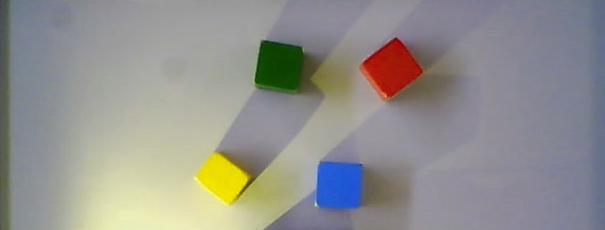
\includegraphics[scale=0.3]{images/cropped}
		\caption{Billede skåret til bordpladen}
		\label{fig:cropped}
	\end{subfigure}
	\begin{subfigure}{.45\textwidth}
		\centering
		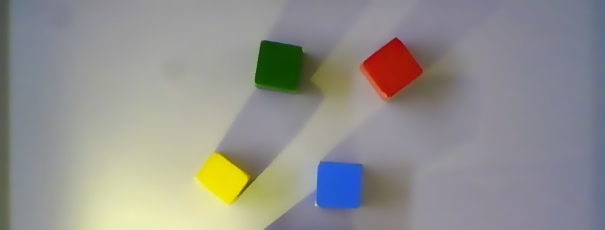
\includegraphics[scale=0.3]{images/smooth}
		\caption{Udglattet billede}
		\label{fig:smooth}
	\end{subfigure}
	\caption{Preprocessering}
	\label{fig:preprocessing}
\end{figure}


Nu bruges en canny edge detektor til at finde kanterne i billedet (Se figur \ref{fig:canny}).
Kanterne er ikke sammenhængende, men blot nogle pixels der er blevet markeret som værende en del af en kant. \\

For at samle disse pixels til en sammenhængende kant bruges en morfologisk transformation (Se figur \ref{fig:close}).
Closing, der består af dilation efterfulgt af erosion, bruges til at lukke huller imellem pixels. \\

\begin{figure}[H]
	\centering
	\begin{subfigure}{.45\textwidth}
		\centering
		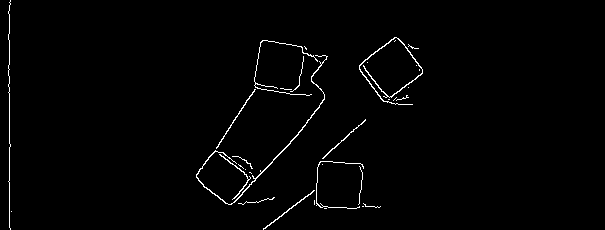
\includegraphics[scale=0.3]{images/canny}
		\caption{Resultat af Canny edge detection.}
	  	\label{fig:canny}
	\end{subfigure}
	\begin{subfigure}{.45\textwidth}
		\centering
		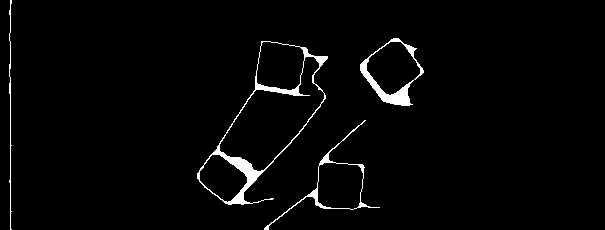
\includegraphics[scale=0.3]{images/closed}
		\caption{Resultat efter closing.}
		\label{fig:close}
	\end{subfigure}
	\caption{Edge detection}
	\label{fig:edges}
\end{figure}

For at finde klodserne ud fra billedet, bruges findContours metoden (Se figur \ref{fig:contours}).
Den giver en liste af alle konturer og deres hierarki som en træstruktur.
For at finde klodserne ud fra konturerne er der lavet en rekursiv metode der går træet igennem og finder konturer.
Når en konturer er identificeret som en klods, søges der ikke dybere i træet.
Det skyldes at de tykke kanter i billedet kan blive til to konturer, én på ydersiden og én på indersiden af kanten.
Uden at kigge på hierakiet ville en klods derfor blive identificeret to gange. \\

Selve identifikationer af en klods ud fra en kontur, gøres ved at kigge på forskellige egenskaber af konturen (Se figur \ref{fig:blocks}).
Der kigges på arealet af konturen da det vides hvilket interval klodsernes areal ligger indenfor.
Der kigges også på længden af konturen, da konturen ikke er en perfekt firkant med fire lige sider.
Til sidst kigges der på forholdet imellem konturens højde og bredde, da vi ved at alle klodserne set oppe fra er næsten kvadratiske.
Hvis forholdet er 1 er figuren kvadratisk. \\

Klodsernes hjørner bruges videre i systemet til at beregne klodsens orientering og centrum.

\begin{figure}[H]
	\centering
	\begin{subfigure}{.45\textwidth}
		\centering
		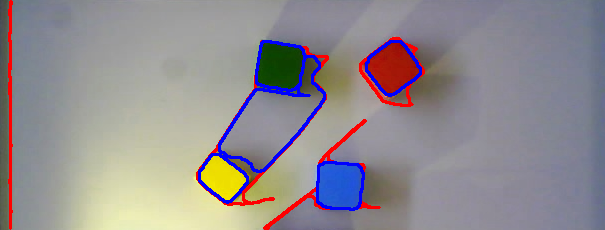
\includegraphics[scale=0.3]{images/contours}
		\caption{Konturernes farve beskriver hierakiet.}
	  	\label{fig:contours}
	\end{subfigure}
	\begin{subfigure}{.45\textwidth}
		\centering
		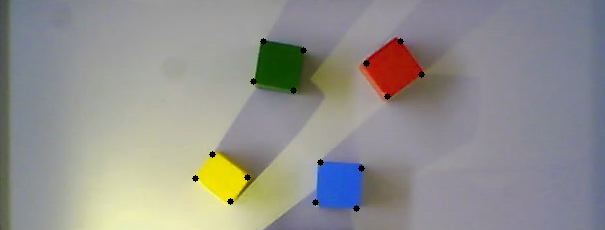
\includegraphics[scale=0.3]{images/blocks}
		\caption{Klodsernes hjørner er markeret.}
		\label{fig:blocks}
	\end{subfigure}
	\caption{Identifikation af klodser ud fra konturer}
	\label{fig:identification}
\end{figure}